\subsection{Long-time data}
\label{sub:long-range}

\todo[review the intro]

This subsection investigates the full archive of match results spanning the last 20 seasons of English volleyball. The focus here is on identifying macro-level patterns, such as dominant teams over time, seasonal win-loss distributions, changes in competitive balance, and the evolution of game dynamics. A series of charts and graphs will support this analysis, offering visual representations of league trajectories, performance cycles, and notable statistical anomalies. By establishing a long-term view, this analysis sets the stage for comparisons with present-day developments.

\subsubsection{Points Distribution}
By plotting the number of total points in a game (i.e. the sum of all the points scored by both teams) we can get an idea of what an average game looks like.

Figure \ref{fig:point-histogram} shows the point distribution by sex. The men data is slightly shifted to the right, which indicates that men games tend to have more points in total. This could mean that the level among men teams is more homogeneous than in women teams. However, the difference is not significative.

\begin{figure}
	\centering
	\subfloat[Points by category]{{
			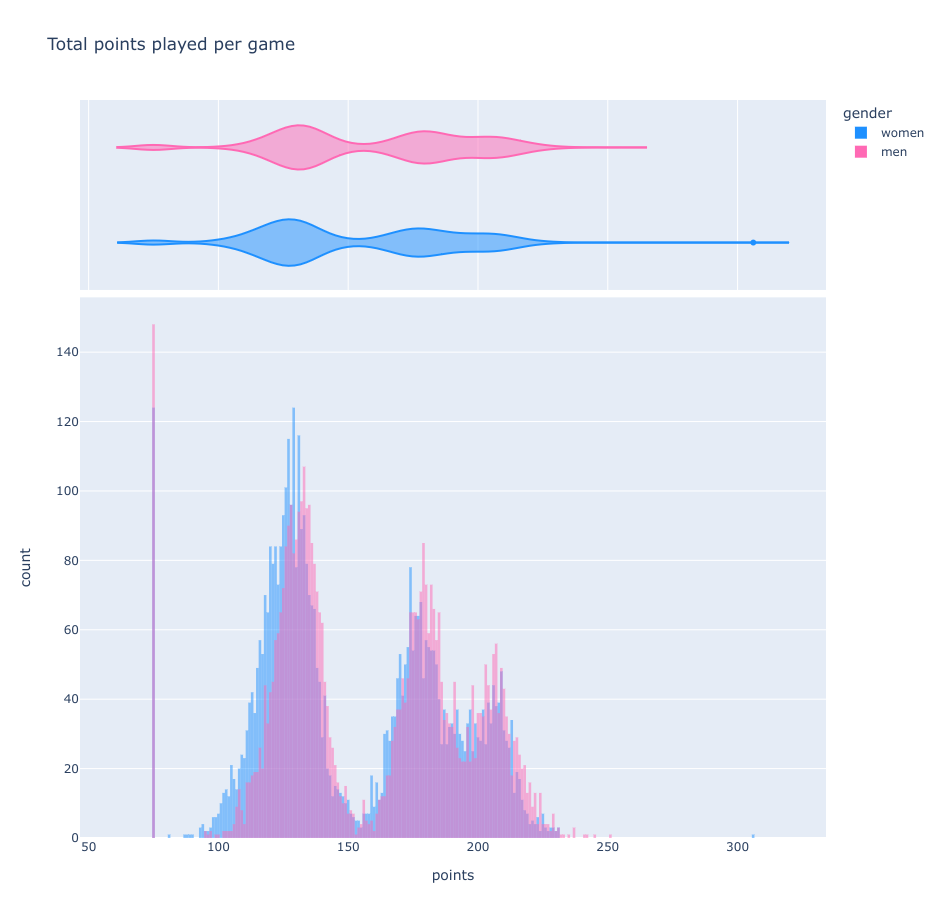
\includegraphics[width=.4\linewidth]{points-histogram-sex.png}
	}}
	\qquad
	\subfloat[Points by number of sets]{{
			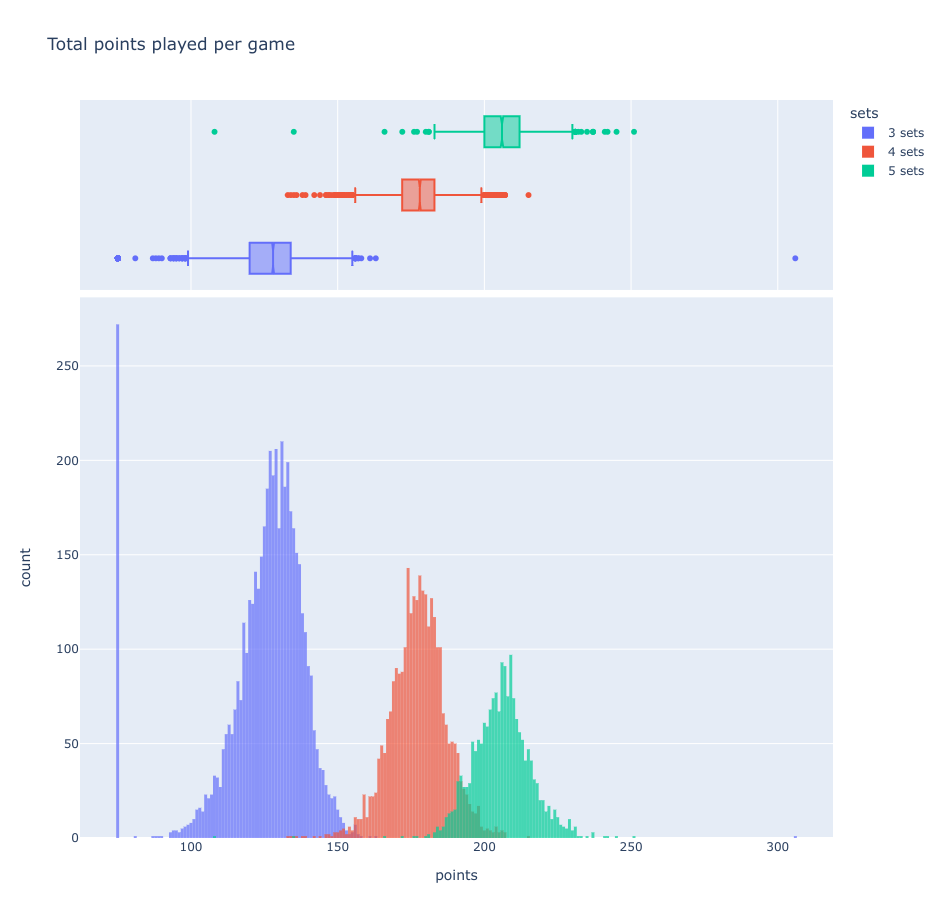
\includegraphics[width=.4\linewidth]{points-histogram-sets.png}
	}}
	
	\caption{Histograms showing the distribution of the total match points}
	\label{fig:point-histogram}
\end{figure}

The lonely column on the far left are the games with a total point sum of 75. These can only happen if the result is 25-0 25-0 25-0, which indicates a forfeit. The chart shows that men tend to forfeit around 25\% more than women, with 146 games forfeited by men, versus 116 by women.

The 3 peaks that can be observed in the histogram correlate to the number of sets. This can be better observed in figure \ref{fig:point-histogram}. In blue are the games that were just 3 sets long. This includes the forfeits, prominently displayed on the left again. As expected, the number of 3-set games is greater than the number of 4-set games, which is in turn greater than the number of 5-set games.

We can also observe that the overlap in the number of points between 3 and 4 set games is much smaller than the overlap between 4 and 5 set games. This is of course due to the 5\textsuperscript{th} set being capped at 15 points.

The games seem to follow a normal distribution, meaning that extreme results --such as 25-3, for example-- are quite rare; and on average, teams are evenly matched.

\subsubsection{Game Results}
As stated earlier, 3-set games are the most common by far, accounting for ~52\% of the results. Games to 4 sets add up to ~30\% of the outcomes, while only ~18\% of games reach the tie-breaker.
Of those results, most of the times a home victory is expected 55\% of times, indicating that a familiar environment does actually cause some effect --albeit only marginally--. Breaking down these findings by division, we can see that the higher the division, the more important it seems to be to play "at home", as shown in figure \ref{fig:home-victories-per-division}. I was really not expecting this, since I assumed that higher level players would be more\ldots professional, for lack of a better word, and they would be impervious to environment changes.

Some of these games are played in neutral ground (e.g. the Cup finals), which might skew the results a bit. However, the amount of these occurrences is too small to be significative, so no further refinement was made.

\begin{figure}
	\centering
	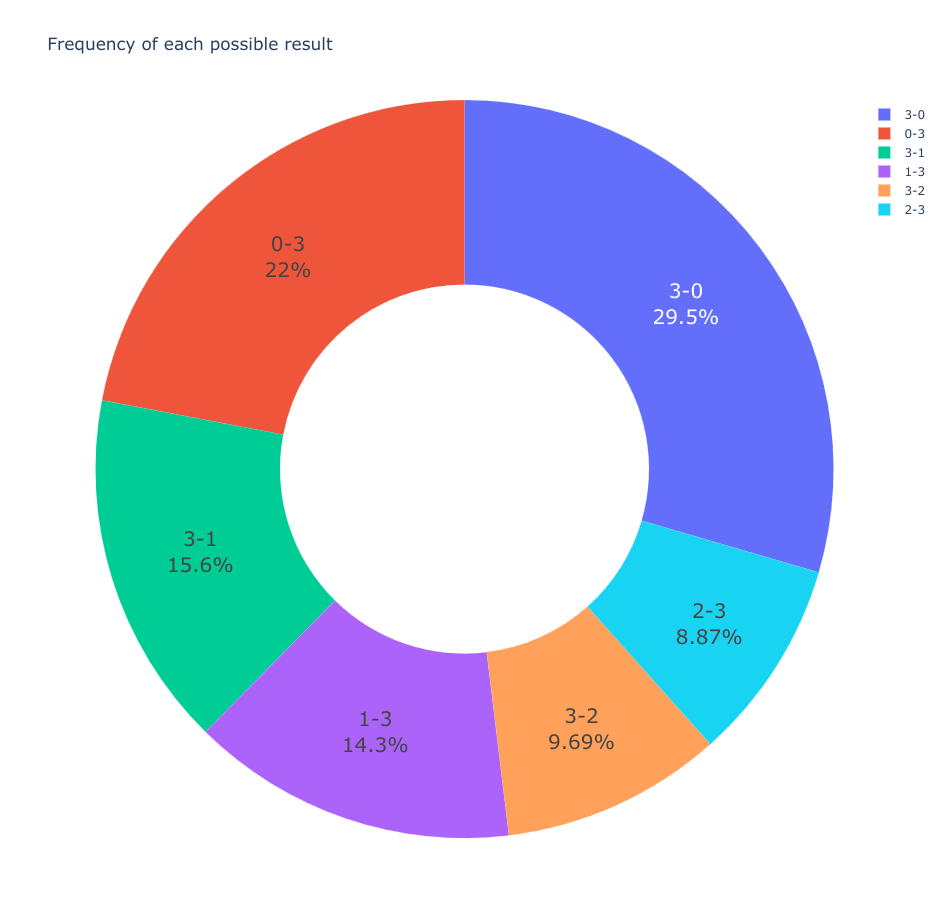
\includegraphics[width=.7\linewidth]{results-pie-chart.png}
	\caption{Frequency of each possible result}
	\label{fig:results-pie-chart}
\end{figure}

\begin{figure}
	\centering
	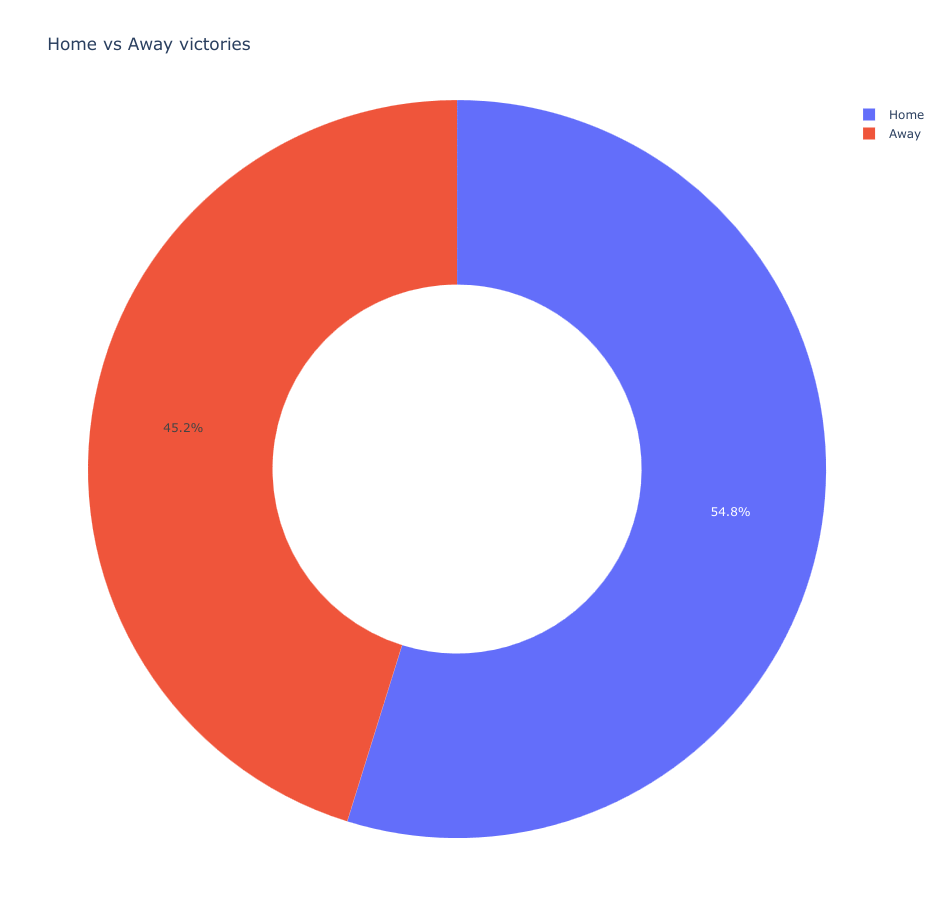
\includegraphics[width=.7\linewidth]{home-away-victories.png}
	\caption{Number of home vs away victories}
	\label{fig:home-away-victories}
\end{figure}

\begin{figure}
	\centering
	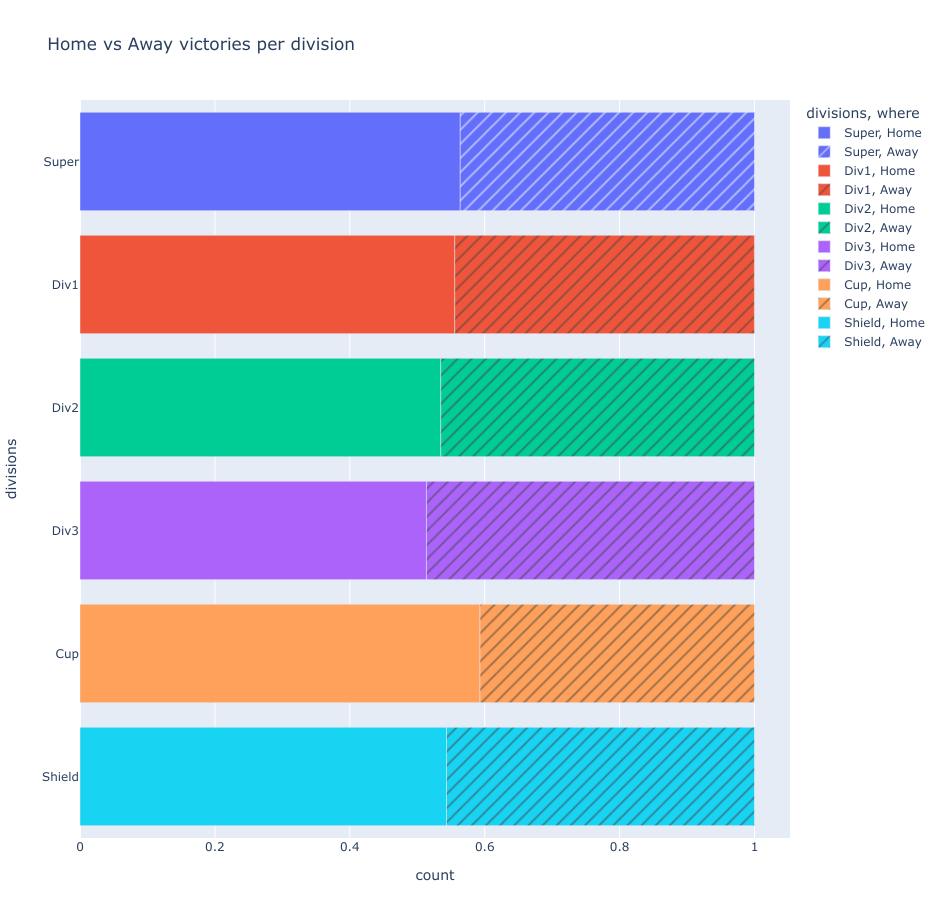
\includegraphics[width=.7\linewidth]{home-victories-per-division.png}
	\caption{Percentage of home victories, split by division}
	\label{fig:home-victories-per-division}
\end{figure}


\subsubsection{Evolution}
\ac{VE} has clearly been working to promote, develop and grow the sport in England, and the following charts are proof of it. Figure \ref{fig:games-per-year} plots the number of games each season, showing a massive increase since 183 games in 2005 to +1200 in 2025. That means a 7-fold increment. Particularly noticeable is the effect of COVID lockdown: there were no games in the 2020/2021 season, and the 2021/2022 season had to be cut short early, due to additional lockdown measures.

\begin{figure}
	\centering
	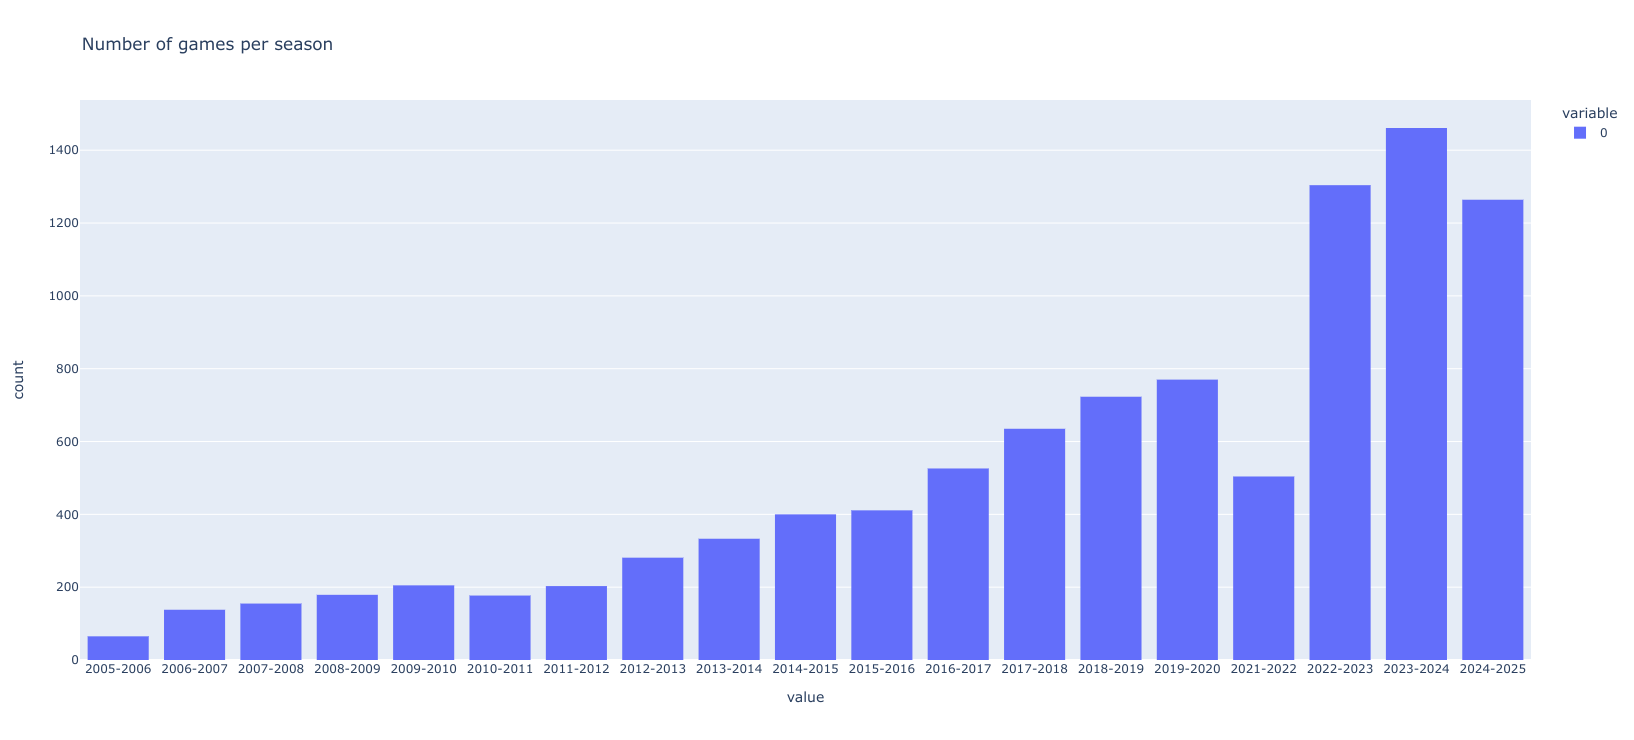
\includegraphics[width=0.7\linewidth]{games-per-year.png}
	\caption{Total number of games each season}
	\label{fig:games-per-year}
\end{figure}

If we split by division, shown in figure \ref{fig:games-per-year-by-division}, we can see the start of the Superleague (Super8) back in 2010. More importantly, we can see that the increase in the number of games has come mainly from a corresponding increase in Division 2 and specially Division 3, particularly since 2022.

\begin{figure}
	\centering
	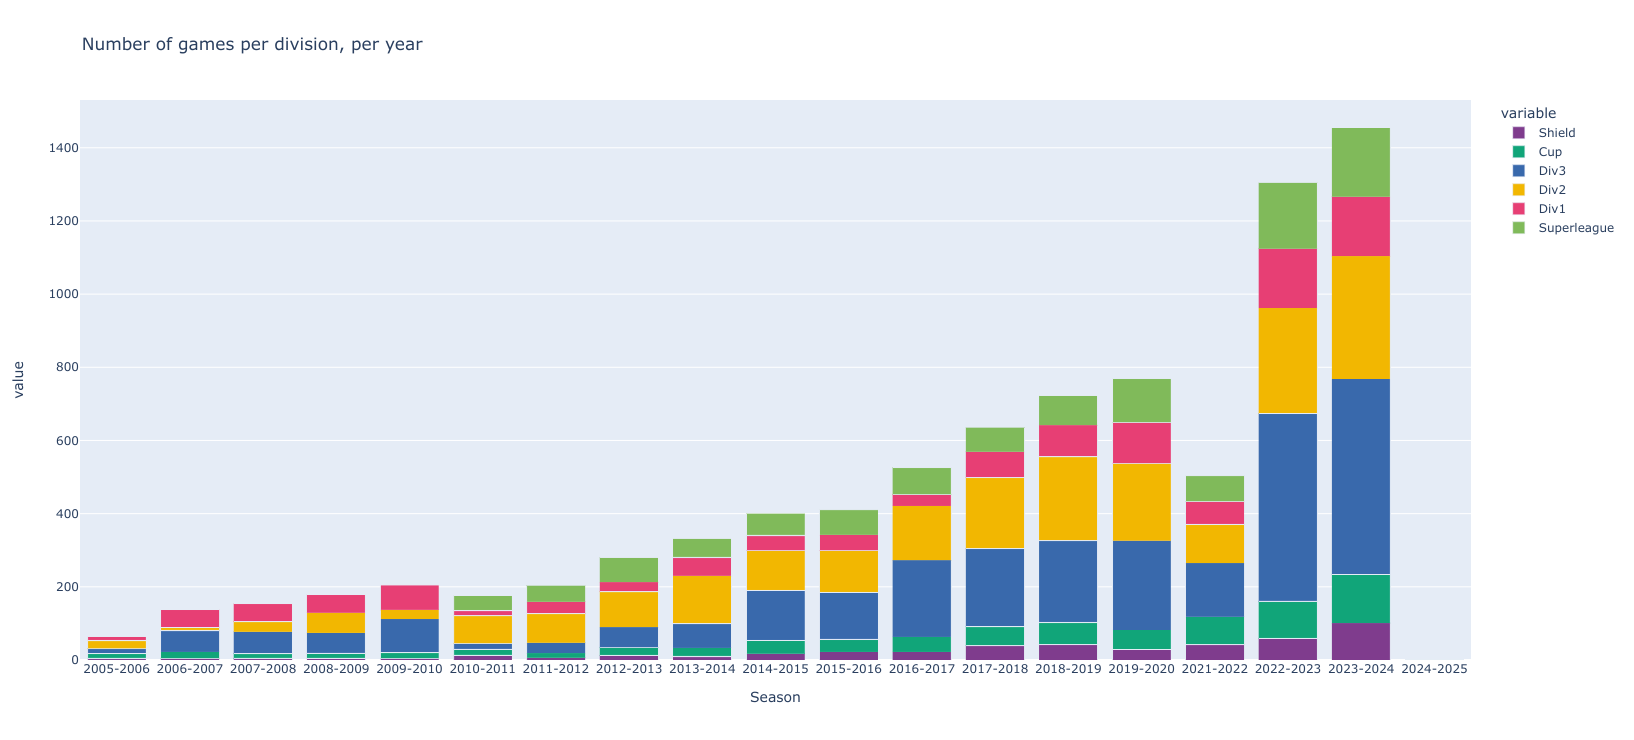
\includegraphics[width=0.7\linewidth]{games-per-year-by-division.png}
	\caption{Total number of games each season, split by division}
	\label{fig:games-per-year-by-division}
\end{figure}

One would expect these increments to be caused by a similar increase in the number of teams. However, figure \ref{fig:teams-per-year} shows that te biggest increments have happened in the Cup and Shield competitions, specially in the last couple of seasons.

\begin{figure}
	\centering
	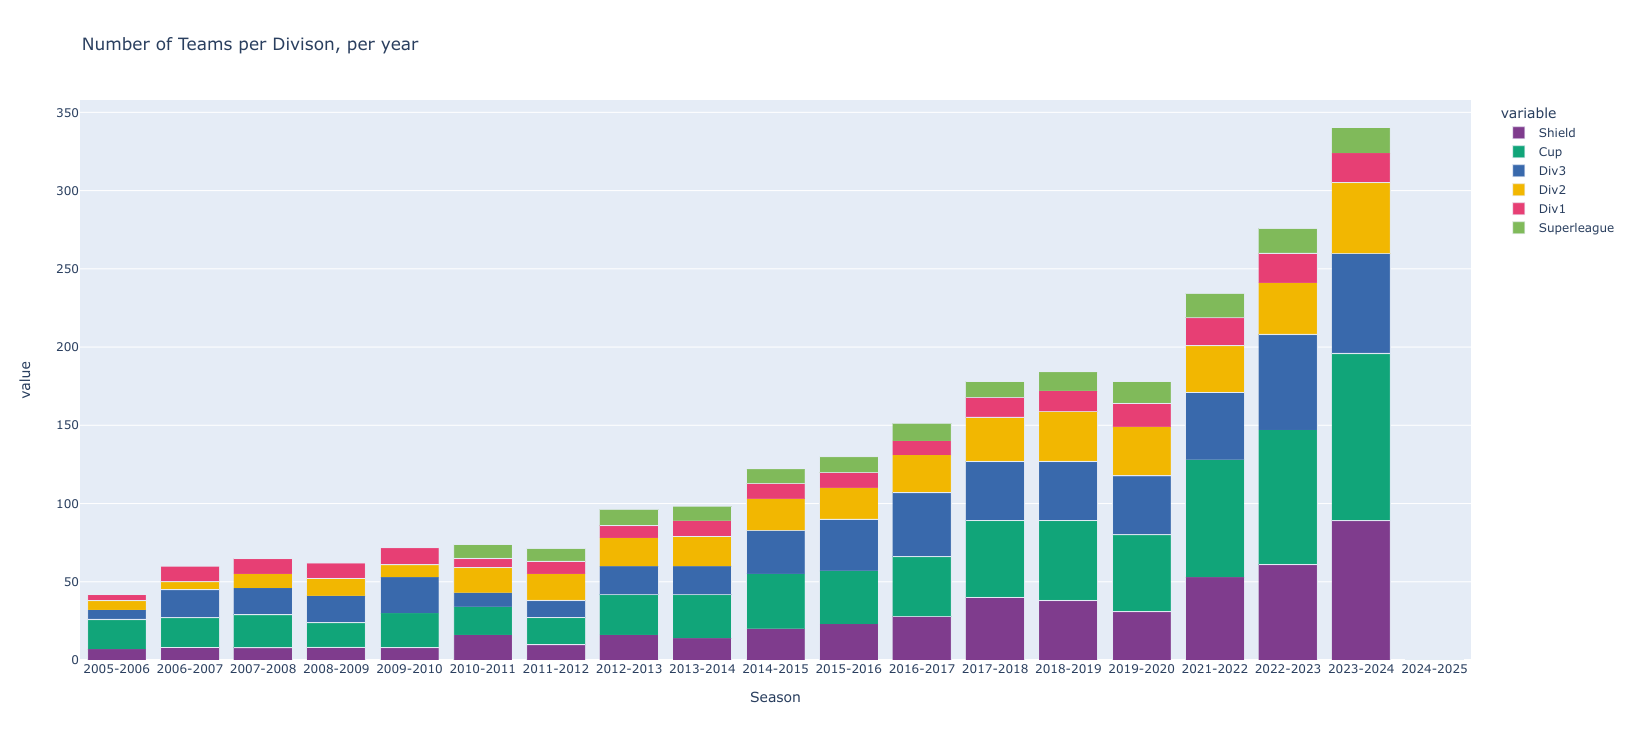
\includegraphics[width=0.7\linewidth]{teams-per-year.png}
	\caption{Number of teams competing in each division every season}
	\label{fig:teams-per-year}
\end{figure}
